\documentclass[a4paper,11pt]{scrreprt}

\usepackage[utf8]{inputenc}
\usepackage{amsthm}
\usepackage{amssymb}
\usepackage{ngerman}
\usepackage{graphicx}
\usepackage{textcomp}
\usepackage{gensymb}
\usepackage{float}

\setlength{\parindent}{0pt}
\setlength{\parskip}{0.8em}

\title{Reoptimierung am Beispiel des TSP}
\subtitle{Seminararbeit Theoretische Informatik 6. Semester}
\author{Florian Müller, flm@fastmailfm, ZHAW}
\date{}

\begin{document}

\maketitle

\begin{abstract}
\end{abstract}

\tableofcontents

\chapter{Einleitung}

In dieser Arbeit wird anhand des Travelling Salesman Problems (TSP) aufgezeigt,
inwiefern eine bereits gefundene optimale Lösung wiederverwendet werden kann,
um eine minimal veränderte Probleminstanz zu approximieren. 

\chapter{Grundlagen}

Da die Zielgruppe dieser Arbeit Studenten sind, werden gewisse Grundlagen, welche danach für das Verständnis der Beweisführungen wichtig sind, in diesem Kapitel nochmals kurz aufgefrischt.

\section{TSP- Travelling Salesman Problem}

Das Travelling Salesman Problem (TSP) besteht aus einer Probleminstanz $(G, c)$,
wobei $G = (V, E)$ ein vollständiger ungerichteter Graph und $c = E \rightarrow \mathbb{R}^+$ eine Kostenfunktion ist, welche jeder Kante in $E$ eine reelle Zahl
zuordnet. Gesucht wird die Tour $T = (v_1, \dots, v_n, v_1)$ von einem
Startknoten $v_1$ aus durch alle anderen Knoten zurück zum Startknoten mit minimalen Kosten. 

\section{Hamilton-Pfad und Hamilton-Kreis}

Ein Hamilton-Pfad $HP$ ist ein Pfad durch eine Menge von Knoten $V = {v_1, \dots, v_n}$, welcher einmal durch jeden Knoten geht ($HP = (v_1, \dots, v_n)$) und jede Kante höchstens einmal benutzt.

Ein Hamilton-Kreis $HC$ geht wie der Hamilton-Pfad einmal durch jeden Knoten, muss jedoch im selben Knoten enden, bei dem er gestartet ist ($HC = (v_1, \dots, v_n, v_1)$).

\section{Polynomialzeit-Reduktion}

Eine Polynomialzeit-Reduktion ($\prec$) ist der Prozess, bei dem jede Probleminstanz eines Problems $P_A$ in Polynomialzeit in eine gültige Probleminstanz des Problems $P_B$ umgewandelt werden kann. Das heisst, die 
Reduktion ist eine Funktion $f(I_A) \rightarrow I_B$. Zudem gilt, dass falls
eine Lösung für $I_A$ existiert, auch eine Lösung für $I_B$ existiert und umgekehrt.

In dieser Arbeit wird die Reduktion von NP-vollständigen Problemen auf Probleme
der Reoptimierung benutzt, um zu beweisen, dass diese Probleme NP-schwer sind.

Eine Reduktion in dieser Arbeit hat immer die Form 

$Problem_{NP-vollst"andig} \prec Problem_{zu beweisen NP-schwer}$ 

und eine erfolgreiche Reduktion sagt aus, dass $Problem_{zu  beweisen NP-schwer}$ mindestens so schwer ist wie $Problem_{NP-vollst"andig}$.

Damit werden wir beweisen, dass auch Reoptimierungsprobleme NP-schwer sind und daher kein Polynomialzeit-Algorithmus dafür existiert (ausser $P = NP$).

\section{Metrisches TSP}

Das metrische TSP ist ein Spezialfall des TSP, welches die Dreiecksungleichung erfüllt. Diese besagt, dass der direkte Weg von einem Knoten zu einem anderen immer kleiner oder gleich ist, wie der Umweg über zwei andere Kanten. Formal:

$c({u, w}) \le c({u, v}) + c({v, w})$

wobei $c$ die Kostenfunktion $c: E \rightarrow \mathbb{R}+$ ist, welche jeder Kante Kosten zuordnet.

Dies entspricht den geometrischen Gegebenheiten. Man muss sich das vorstellen,
wie in Abbildung \ref{fig:trangle-inequality}. Die Kante $c$ kann nur grösser 
werden, indem man den Winkel zwischen $a$ und $b$ vergrössert. Dies kann man 
höchsten so lange machen, bis der Winkel $180^\degree$ beträgt und $c = a + b$, danach
wird $c$ wieder kleiner.

\begin{figure}
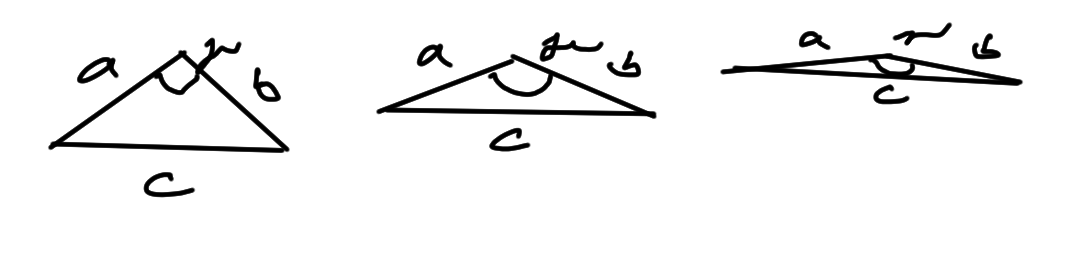
\includegraphics[width=0.8\textwidth]{triangle_inequ.png}
\caption{Dreiecksungleichung}
\label{fig:trangle-inequality}
\end{figure}

\section{TSP mit Deadlines}

\chapter{Reoptimierung des TSP}

\section{Definitionen}

Dieses Kapitel behandelt drei Arten von Travelling Salesman Problemen:

\begin{description}
\item[$lm-TSP$] 
Beschreibt das Problem, das als Eingabe einen vollständigen Graphen $G = (V, E)$, eine originale Kostenfunktion $c_O$, eine optimale Tour $\overline{C}$ und eine modifizierte Kostenfunktion $c_N$ bekommt und daraus eine neue optimale Tour $C$ ermitteln soll. Die Kostenfunktion $c_N$ ist so konstruiert, dass sie genau für eine Kante $e$ einen anderen und für alle $E \backslash \{e\}$ denselben Wert wie $c_o$ ausgibt. Formal lautet eine Probleminstanz $I$ für $lm-TSP$ demnach $I = (G, c_O, c_N, \overline{C})$.
			    
Die Knoten- und Kantendefinitionen ändern sich dabei nicht.

\item[$lm-\triangle_\beta-TSP$]
Ist ein Spezialfall des $lm-TSP$ für Kostenfunktionen $c$, welche folgende Dreiecksungleichung erfüllen:

\[ c(\{u,w\}) \le \beta \cdot (c(\{u,v\} + c(\{u,w\}))) \]

Für das metrische TSP $\triangle_1-TSP$ wird als Abkürzung $\triangle-TSP$ verwendet.

Falls $\beta < 1$ wird von einer verschärften, falls $\beta > 1$ von einer abgeschwächten Dreiecksungleichung gesprochen (siehe Abbildung \ref{fig:triangle-inequality-beta}).

\begin{figure}[H]
\centering
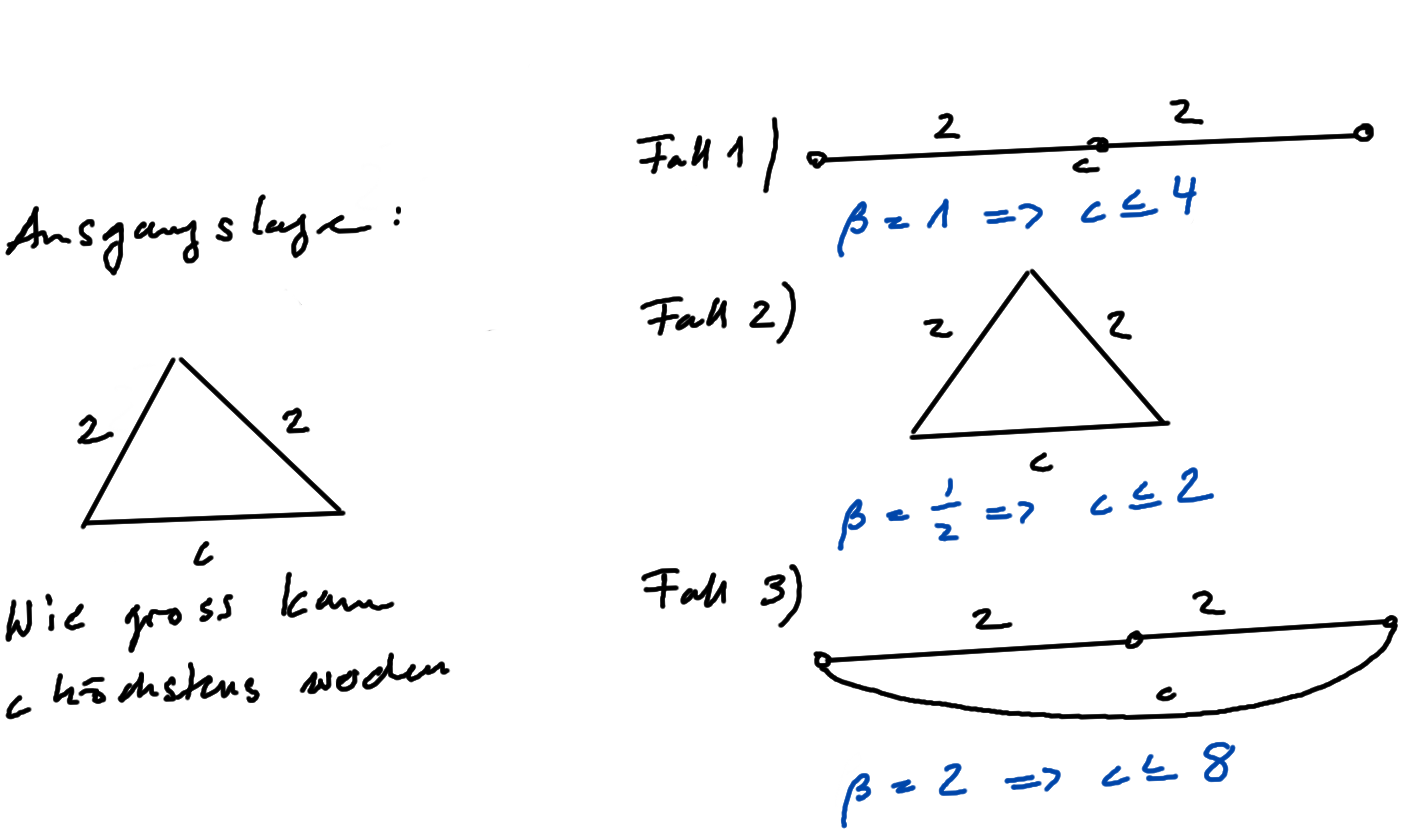
\includegraphics[width=0.6\textwidth]{triangle_inequality_beta.png}
\caption{Dreiecksungleichung mit verschiedenen $\beta$}
\label{fig:triangle-inequality-beta}
\end{figure}

\item[$lm-DL-TSP$]

Das $lm-DL-TSP$ bezieht sich auf TSPs mit Deadlines, welche in den Grundlagen bereits erklärt sind.

Als lokale Modifikation wird bei Deadline-TSPs die Veränderung genau einer Deadline betrachtet. $lm-DL-TSP$ soll unter Berücksichtigung der neuen Deadlines eine neue optimale Tour berechnen.

Die Probleminstanz $I$ kann formal als $I = (G, D, c, d_O, d_N, \overline{C})$ beschrieben werden, wobei $G = (V, E)$ den Graphen darstellt, $D = \{v_1, \dots, v_k \}$ die Deadline-Knoten, $c: E \rightarrow \mathbb{R}^+$ die Kostenfunktion, welche für beide Probleme gilt, $d_O: D \rightarrow \mathbb{R}^+$ die originale Funktion, welche jedem Deadline-Knoten eine Deadline zuordnet und $d_N: D \rightarrow \mathbb{R}^+$ die neue Deadline-Funktion, welche genau einem Knoten eine andere Deadline zuordnet als $d_O$. Gesucht wird die optimale Tour $\overline{C}$ unter Berücksichtigung von $d_N$.

\end{description}

\section{Ziele}

Es ist allgemein bekannt, dass falls $P \not= NP$, es keinen polynomiellen Approximationsalgorithmus mit konstanter relativer Güte r für das allgemeine TSP (ohne Einschränkungen) gibt. Das heisst, eine Garantie, dass das Verhältnis $g = \frac{Solution_{found}}{Solution_{optimal}}$ für jede Eingabe kleiner gleich einem bestimmten \emph{konstanten} Wert $r$ ist (wie z.B. $\frac{3}{2}$).

Wir zeigen anhand eines Beweises von H.-J.-Böckenhauer et. al. (\cite{bok1}), dass dies auch für $lm-TSP$ gilt. Das heisst, das Problem wird nicht leichter, obwohl die Änderung nur eine einzige Kante betrifft und eine optimale Lösung für das Originalproblem bereits ermittelt wurde.

Des weiteren wird gezeigt, dass das Problem einfacher wird, wenn wir fordern, dass die $\beta-$-Dreiecksungleichung eingehalten werden muss. Daraus ergibt sich das Problem $lm-\triangle_\beta-TSP$. H.-J. Böckenhauer et. al. (\cite{bok1}, \cite{bok2}) konnten für eine Teilklasse dieser Probleme mit $\beta > \frac{1}{2}$ zeigen, dass dieses Problem weiterhin NP-schwer ist, dass jedoch ein polynomieller Approximationsalgorithmus mit konstanter relativer Güte existiert, welche nur vom Parameter $\beta$ abhängt. Die relative Güte verbessert sich im metrischen Fall $lm-\triangle_1-TSP = lm-\triangle-TSP$ gegenüber der bisher durch den Algorithmus von Christofides erreichten 1.5 auf 1.4 und schlägt auch im Bereich von $1 < \beta < 3.34899$ alle bisher bekannte Algorithmen (\cite{bok1} S. 253).

Schlussendlich wird anhand H.-J. Böckenhauer et. al. (\cite{bok2}) bewiesen, 
dass im Fall des TSP mit Deadlines $LM-DL-TSP$ jeder polynomielle Approximationsalgorithmus für die relative Güte eine untere Schranke von $(2-\epsilon)$ für jedes $\epsilon > 0$ nicht unterschreiten kann. Diese Schranke gilt auch für das Originalproblem $DL-TSP$, was uns zeigt, dass wir im Fall von $LM-DL-TSP$ keinen Vorteil daraus gewinnen können, dass wir bereits eine Lösung für das Originalproblem kennen.

Alle Beweise basieren auf den Arbeiten \cite{bok1} und \cite{bok2} von H.-J. Böckenhauer et. al.

\section{Die Schwere von $LM-TSP$}

\newtheorem{t1}{Theorem}

\begin{t1}
Es gibt für $LM-TSP$ keinen polynomiellen Approximationsalgorithmus (ausser $P = NP$).
\end{t1}

\begin{proof}[Beweis]
Dazu führen wir eine Reduktion vom Hamilton-Kreis $HC$ Problem auf $LM-TSP$ durch.

\[HC \prec LM-TSP \]

\textbf{Hamilton-Kreis-Problem} Es ist ein ungerichteter Graph $G = (V, E)$ mit $V = \{v_1, \dots, v_n\}$ und $E = \{e_1, \dots, e_k\}$ ohne Kantengewichte gegeben. Gesucht wird die Entscheidung, ob $G$ ein Hamilton-Kreis besitzt oder nicht.

\textbf{Reduktion} Der ungerichtete Graph $G$ wird zuerst in einen ungerichteten \emph{vollständigen} Graphen $G_O = (V', E')$ mit einer Kostenfunktion $c_O$ umgewandelt. Dieser Graph wird so konstruiert, dass eine optimale Tour $\overline{C}$ offensichtlich ist. Danach werden die Kosten einer einzigen Kante so verändert (neue Kostenfunktion $c_N$), dass die Tour $\overline{C}$ nicht mehr optimal ist. Eine weitere optimale Tour entspräche nun genau einem Hamilton-Kreis in G und umgekehrt: ein Hamilton-Kreis in G entspräche genau einer optimalen Tour in $G_O$ unter der neuen Kostenfunktion $c_A$. 

\textbf{Schritt 1} Für jeden Knoten $v_i \in V$ wird ein sogenannter Diamant-Graph erstellt. Alle Kantenkosten sind dabei genau 1. (Abbildung \ref{fig:lm-tsp-proof-step1}). Die Bezeichner ${N_i, E_i, S_i, W_i}$ stehen dabei für north, east, south und west. Das Spezielle an diesen Diamantgraphen ist, dass sie so konstruiert sind, dass es genau zwei Wege durch sie hindurch gibt, möchte man jeden Knoten genau einmal besuchen. 1) West $\rightleftarrows$ Ost 2) Nord $\rightleftarrows$ Süd (Abbildung \ref{fig:lm-tsp-proof-step1-ways}). Diese Tatsache wird hier nicht bewiesen.

\begin{figure}[H]
\centering
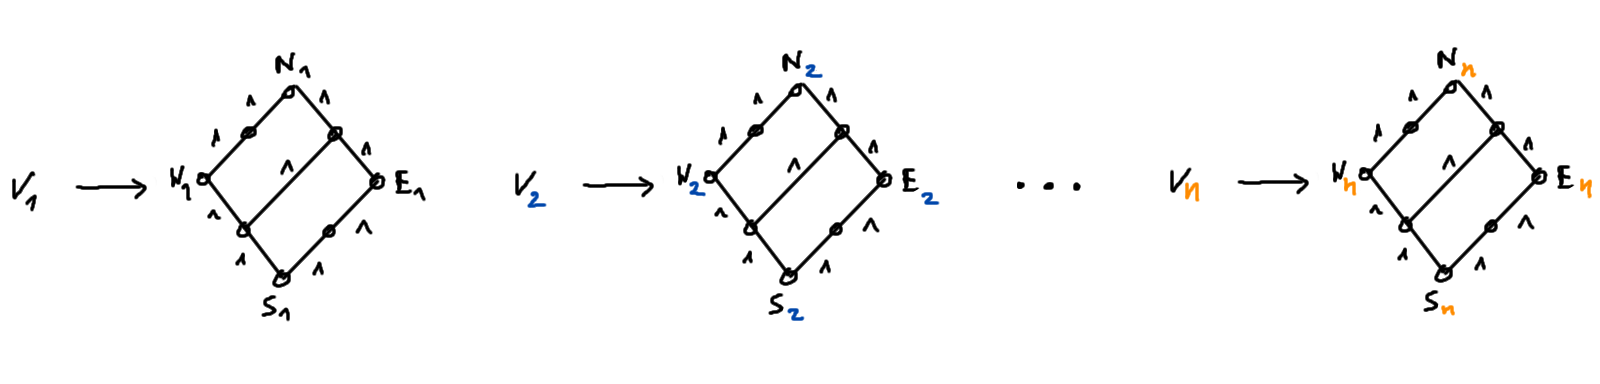
\includegraphics[width=0.9\textwidth]{lm_tsp_proof_step1.png}
\caption{Im ersten Schritt werden alle Knoten aus $V = \{v_1, \dots, v_n \}$ in einen Diamant-Graphen mit allen Kantenkosten = 1 umgewandelt}
\label{fig:lm-tsp-proof-step1}
\end{figure}

\begin{figure}[H]
\centering
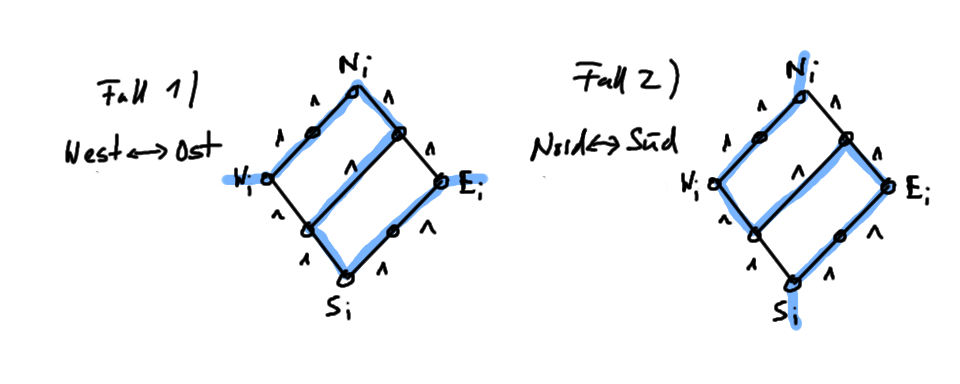
\includegraphics[width=0.6\textwidth]{lm_tsp_proof_step1_ways.png}
\caption{Es existieren genau zwei Wege durch den Diamanten hindurch, möchte man jeden Knoten genau einmal besuchen}
\label{fig:lm-tsp-proof-step1-ways}
\end{figure}

\textbf{Schritt 2} Wir definieren $M := n \cdot 2^n + 1$ in Abhängigkeit der Anzahl Knoten in $G$ $|V| = n$. Die einzelnen Diamant-Graphen werden wie auf Abbildung \ref{fig:lm-tsp-proof-step2} zu einem vollständigen Graphen $G_O = (V', E')$ zusammengeführt. Alle Kanten $\{E_i, E_{i+1}\}$ und ausserdem die Kante $\{E_n, E_1\}$ erhalten die Kosten $1$. 

Alle Kanten $\{S_i, N_j\}$ (alle Verbindung zwischen dem $S$-Knoten des einen Diamanten mit dem $N$-Knoten eines anderen Diamanten) erhalten die Kosten $1$ genau dann, wenn $\{v_i, v_j\} \in E$, das heisst, wenn diese Kante bereits im Originalgraphen $G = (V, E)$ vorhanden war. Falls nicht, erhalten sie die Kosten $M$. 

Da $G_O$ ein vollständiger Graph ist, existieren noch viele weitere Kanten (jeder Knoten muss mit jedem anderen Knoten verbunden werden); jede dieser Kanten erhält auch die Kosten $M$. 

Die optimale Tour $\overline{C}$ ist in Abbildung \ref{fig:lm-tsp-proof-step2} eingetragen. Die Kosten $c_O(\overline{C})$ betragen genau $8 \cdot n$ ($7 \cdot n$ in jedem Diamanten plus jeweils die Verbindung \emph{zwischen} den Diamanten).

\begin{figure}[H]
\centering
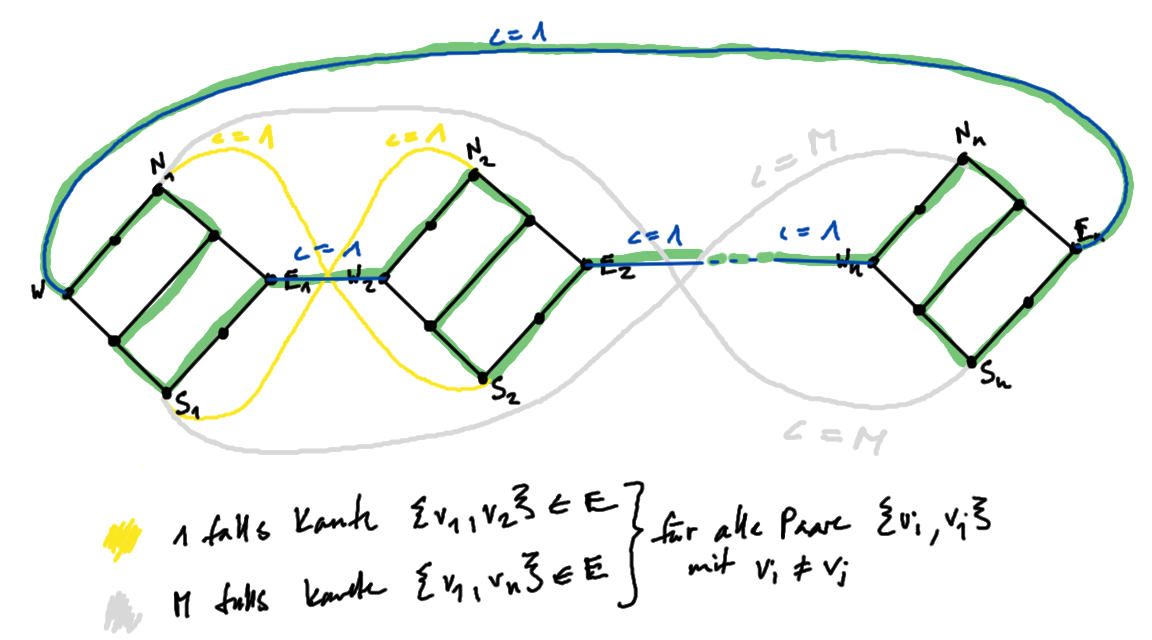
\includegraphics[width=0.8\textwidth]{lm_tsp_proof_step2.png}
\caption{}
\label{fig:lm-tsp-proof-step2}
\end{figure}

\textbf{Schritt 3} Damit ein Problem der Form $LM-TSP$ geschaffen werden kann, werden die Kosten genau einer Kante angepasst. Kante $\{E_N, W_1\}$ erhält neu die Kosten $M$. Die bisherige Lösung hat nun die Kosten $c_A(\overline{C}) = 8 \cdot n + M - 1$. Eine optimale Lösung hätte erneut auch unter der Kostenfunktion $c_N$ die Kosten $8 \cdot n$ und würde sich jeweils von Nord nach Süd durch die Diamanten bewegen wie in Abbildung \ref{fig:lm-tsp-proof-step3} eingezeichnet. Diese Tour hätte jedoch nur Kosten $8 \cdot n$, falls sich ein Hamilton-Kreis im Originalgraphen $G = (V, E)$ befindet (ansonsten wäre es nicht möglich, nur über Kanten mit Kosten $1$ von einem Diamanten zum nächsten zu gelangen).

\begin{figure}[H]
\centering
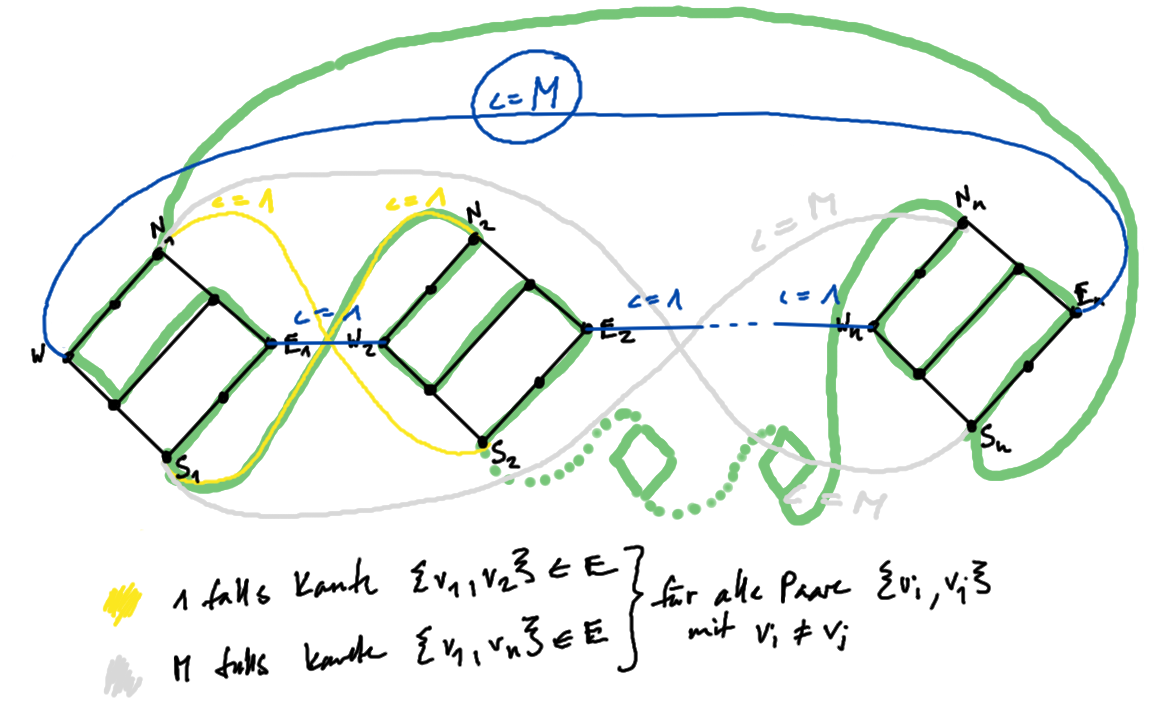
\includegraphics[width=0.8\textwidth]{lm_tsp_proof_step3.png}
\caption{}
\label{fig:lm-tsp-proof-step3}
\end{figure}

\textbf{Schritt 4 - Konklusion} Alle Touren in $G_O$ unter der Kostenfunktion $c_N$, die nicht einem Hamilton-Kreis in $G$ entsprechen, haben im Minimum die Kosten $8 \cdot n - 1 + M$ (eine einzige Verbindung zwischen Diamanten hat anstatt $1$ die Kosten $M$). Das heisst, die relative Güte einer nicht-optimalen Lösung ist im Minimum $\frac{c_A(Solution_{not optimal})}{c_A(Solution_{optimal})}$ = $\frac{8 \cdot n - 1 + M}{8 \cdot n}$ = $\frac{8 \cdot n - 1 + n \cdot 2^n + 1}{8 \cdot n}$ = $1 + \frac{n \cdot 2^n}{n \cdot 2^3}$ = $1 + 2^{n-3}$. Diese Güte ist von n abhängig. D.h. es existiert kein polynomieller Approximationsalgorithmus mit konstanter relativer Güte $r$ für $LM-TSP$.
\end{proof}

\section{$LM-\triangle_\beta-TSP$}

\subsection{Schwere}

Jetzt wo wir gezeigt haben, dass es hoffnungslos ist, für das Problem $LM-TSP$ ein polynomieller Approximationsalgorithmus mit konstanter relativer Güte finden zu wollen (es sei denn $P = NP$), wenden wir uns einer Version des $LM-TSP$, bei welchem die Dreiecksungleichung gilt: das $\triangle_\beta-TSP$. 

Wir könnten nun hoffen, dass $LM-\triangle_\beta-TSP \in P$ und wir daher einen Algorithmus finden können, welcher das Problem in Polynomialzeit exakt löst. Im nächsten Beweis wird gezeigt, dass dies nicht der Fall ist.

\newtheorem{t2}{Theorem}

\begin{t2}
$LM-\triangle_\beta-TSP$ ist NP-schwer für alle $\beta > \frac{1}{2}$
\end{t2}

\begin{proof}[Beweis]
Der Beweis ist eine Reduktion vom Eingeschränkten Hamilton-Kreis Problem (RHC), dargestellt in Abbildung \ref{fig:rhc-reduction-step1}. 

\[ RHC \prec LM-\triangle_\beta-TSP \]

\textbf{RHC} Gegeben ist ein Graph $G = (V, E)$ mit $V = \{v_1, \dots, v_n\}$ und ein Hamilton-Pfad $P = (v_1, \dots, v_n)$, der nicht zu einem Hamilton-Kreis vervollständigt werden kann, indem man einfach die Endpunkte zusammenhängt (wie in Abbildung \ref{fig:rhc-reduction-step1} dargestellt). Gesucht wird nun eine Antwort auf die Frage, ob der Graph $G$ auch einen Hamilton-Kreis enthält. Dieses Problem ist NP-vollständig und wenn uns eine Polynomialzeit-Reduktion auf $LM-\triangle_\beta-TS$ mit $\beta > \frac{1}{2}$ gelingt, wissen wir, dass auch $LM-\triangle_\beta-TS$ mindestens NP-schwer ist.

\begin{figure}[H]
\centering
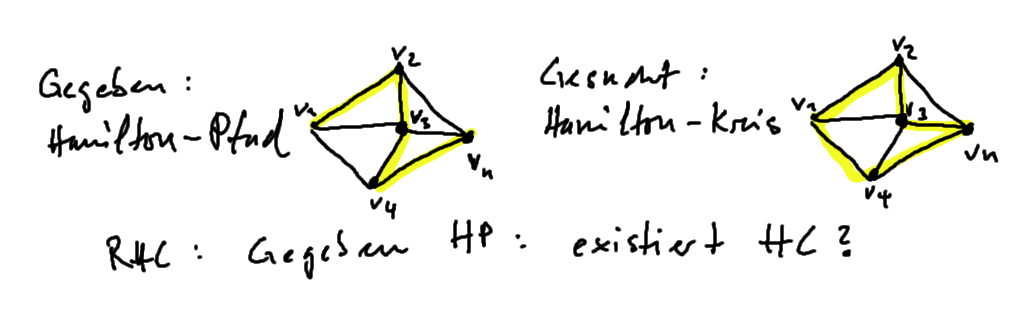
\includegraphics[width=0.8\textwidth]{rhc_reduction_step1.png}
\caption{}
\label{fig:rhc-reduction-step1}
\end{figure}

\textbf{Schritt 1} Wir konstruieren aus $G = (V, E)$ eine Eingabe $I = (G_O, c_N, c_O, \overline{C})$ für $LM-\triangle_\beta-TSP$. Sei $G_O = (V, \tilde{E})$ ein \emph{vollständiger} Graph (mit den gleichen Knoten wie G) und $c_O$ eine Kostenfunktion, welchen einer Kante $e$ den Wert $1$ zuordnet, falls $e$ bereits eine Kante in $G$ war ($e \in E$) oder falls $e = \{v_n, v_1\}$ ist (die Kante, welche im Originalgraphen noch gefehlt hätte, um aus dem Pfad trivialerweise einen Kreis zu machen). Alle anderen Kanten erhalten den Wert $2 \cdot \beta$ (bei $\beta > \frac{1}{2}$ ist dieser Wert immer grösser als $1$). 

\begin{figure}[H]
\centering
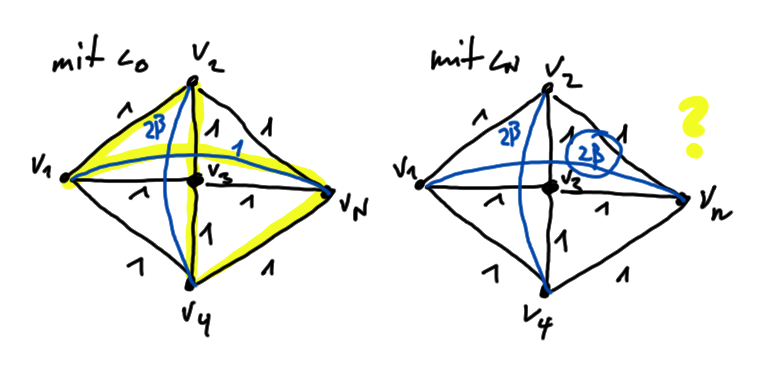
\includegraphics[width=0.6\textwidth]{rhc_reduction_step3.png}
\caption{}
\label{fig:rhc-reduction-step3}
\end{figure}

\textbf{Schritt 2} Die Kostenfunktion $c_N$ unterscheidet sich in genau einer Kante und ordnet der Kante $\{v_n, v_1\}$ anstatt den Wert $1$ den Wert $2 \cdot \beta$ zu. Eine optimale Tour $\overline{C}$ bezüglich $c_O$ ist $\overline{C} = (v_1, v_2, \dots, v_n, v_1)$ (wie in Abbildung \ref{fig:rhc-reduction-step3} links).

\textbf{Schritt 3 - Konklusion} Man kann leicht sehen, dass im Graph $G_O$ unter der Kostenfunktion $c_N$ genau dann eine Tour $C$ mit Kosten $n$ existiert, wenn im ursprünglichen Graph ein Hamilton-Kreis existiert und umgekehrt. Denn nur Kanten, welche im Originalgraphen bereits vorgekommen sind, haben die Kosten 1, alle anderen Kanten haben Kosten $> 1$. 
\end{proof}

\subsection{Ein Approximationsalgorithmus}

Obwohl für $LM-\triangle_\beta-TSP$ kein Algorithmus existiert, der das Problem in Polynomialzeit exakt löst, können wir immer noch auf einen polynomiellen Approximationsalgorithmus mit konstanter relativer Güte hoffen. Tatsächlich haben H.-J. Böckenhauer et. al. (\cite{bok1}, \cite{bok2}) gezeigt, dass es einen solchen Algorithmus gibt, welcher das Problem in Abhängigkeit von $\beta$ (und nicht in Abhängigkeit der Anzahl Knoten $n$) approximiert. Er garantiert eine  relative Güte von

\[ \beta_L\beta_H \cdot \frac{15\beta_L^2 + 5\beta_L - 6}{10\beta_L^2 + 3\beta_L\beta_H + 3\beta_H -6} \]

für Graphenpaare $\{G_O, G_N\}$, so dass $G_O$ die $\triangle_{\beta_O}$-Ungleichung und $G_N$ die $\triangle_{\beta_N}$-Ungleichung erfüllt und $\beta_L := \min(\beta_O,\beta_N)$ und $\beta_H := \max(\beta_O,\beta_N)$. 

Das heisst, die Kostenfunktion $c_O$ ist so konstruiert, dass $c_O(\{u,w\}) = \beta_O \cdot (c_O(\{u,v\}) + c_O(\{v,w\}))$. $c_N$ unterscheidet sich in genau einer Kante und erfüllt die Dreiecksungleichung $c_N(\{u,w\}) = \beta_N \cdot (c_N(\{u,v\}) + c_N(\{v,w\}))$. Beide Graphen $G_O$ und $G_N$ enthalten dieselben Knoten und Kante $V$ und $E$.

\subsubsection{Algorithmus 1}

Der Algorithmus erhält als Eingabe den Graphen $G = (V,E)$, eine originale Kostenfunktion $c_O$, eine optimale Tour unter $c_O$ $\overline{C}$ und eine neue Kostenfunktion $c_N$.

\begin{enumerate}
\item Sei $e \in E$ die Kante im Graphen wo $c_O(e) \not= c_N(e)$ (die Kante, deren Kosten sich verändert haben). Wir stellen nun eine Menge $P$ zusammen, welche ungeordnete Paare von Kanten $\{f, f'\}$ enthält. $f$ und $f'$ sind dabei Kanten, welche direkt an $e$ angehängt sind (siehe Abbildung \ref{fig:lm-beta-approx1}). Dazu unterscheiden wir zwei Fälle:

\begin{description}
\item[Fall 1: $c_O(e) < c_N(e)$] Die Kosten von $e$ sind gestiegen. Wir bilden Paare $\{f, f'\}$ nur unter Kanten, welche sich auf der gleichen Seite von $e$ befinden. Formal: $f \cap f' \cap e$ enthält nur genau $1$ Element (z.B. $\{v_1, v_2\} \cap \{v_1, v_3\} \cap {v_1, v7}$ = $\{v_1\}$ $|\{v_1\}| = 1$).

In Abbildung \ref{fig:lm-beta-approx1} bilden wir im linken Bild nur Paare unter den $f$ und $f'$ Kanten und unter der $g$ und 
$g'$ Kanten.

\item[Fall 2: $c_O(e) > c_N(e)$] Wir bilden Paare $\{f, f'\}$ nur zwischen Kanten, die sich an entgegengesetzten Enden von $e$ befinden und zusammen kein Dreieck bilden. Formal: $f \cup f' = \emptyset$ (z.B. $\{v_1, v_2\} \cap \{v_4, v_7\} = \emptyset)$.

Dies ist in Abbildung \ref{fig:lm-beta-approx1} auf der rechten Seite dargestellt.

\begin{figure}[H]
\centering
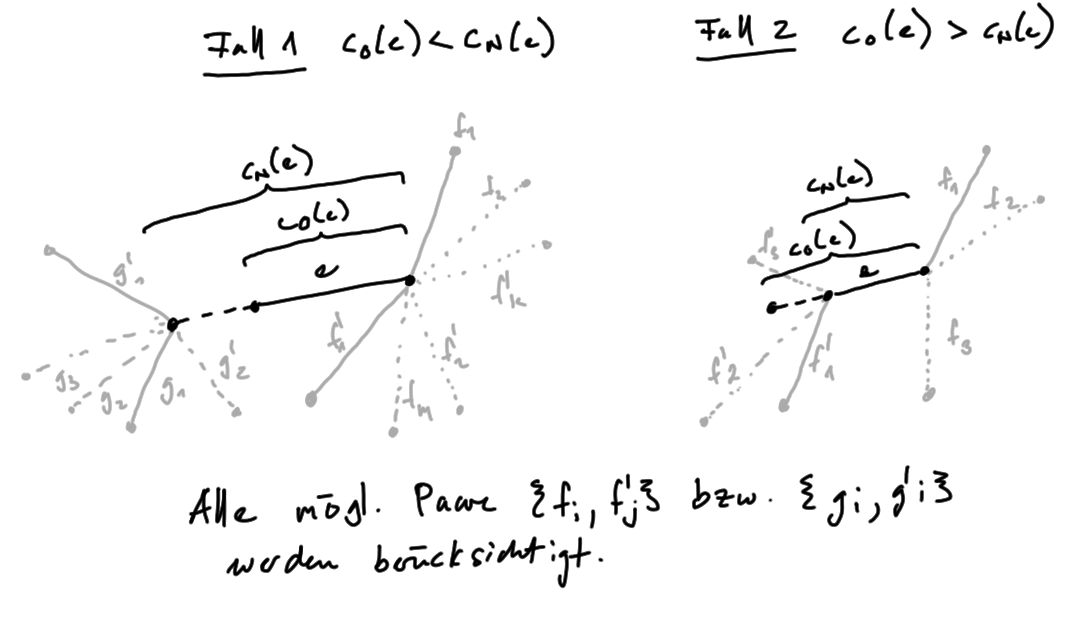
\includegraphics[width=0.9\textwidth]{lm_beta_approx1.png}
\caption{}
\label{fig:lm-beta-approx1}
\end{figure}

\end{description}

\item Danach wird für jedes Paar $\{f, f'\}$ aus $P$ ein Hamilton-Pfad $Q$ zwischen den Knoten aus $f$ und $f'$, welche nicht auch in $e$ vorkommen (formal $(f \cup e)\backslash e$), auf dem Graphen unter Benutzung der Knoten $V\backslash(e\cap(f\cup f'))$ berechnet. Das sind alle Knoten, ausser die, welche $f, f'$ und $e$ gemeinsam haben. Der Pfad $Q$ wird durch die Kanten $f$ und $f'$ und -- falls $c_O(e) > c_N(e)$ (Fall 2) -- durch $e$ ergänzt und bildet so einen Hamilton-Kreis $C_{\{f, f'\}}$. 

Für die Berechnung des Pfades wird ein Algorithmus von Forlizzi et al. verwendet (\cite{for1}).

Der Vorgang ist in Abbildung \ref{fig:lm-beta-approx2} dargestellt.

\begin{figure}[H]
\centering
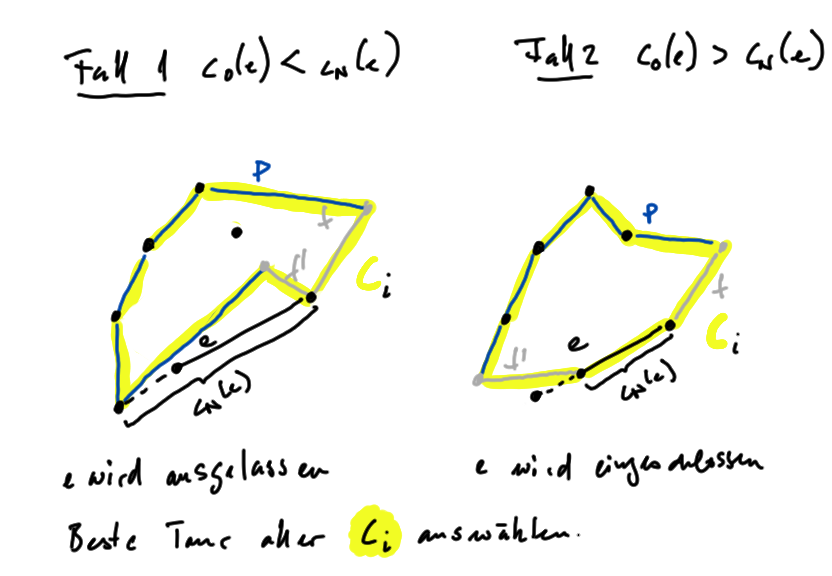
\includegraphics[width=0.9\textwidth]{lm_beta_approx2.png}
\caption{}
\label{fig:lm-beta-approx2}
\end{figure}

\item Im letzten Schritt wählt der Algorithmus die Tour $C$ mit den geringsten Kosten aus der Menge $\{\overline{C}\} \cup \{C_{\{f, f'\}} | \{f, f'\} \in P \}$ (die Menge aller berechneten Touren inklusive der optimalen Tour unter $c_O$) aus.
\end{enumerate}

Der Algorithmus gibt den Hamilton-Kreis $C$ aus.

\begin{thebibliography}{9}

\bibitem{bok1}
  H.-J. Böckenhauer, L. Forlizzi, J. Hromkovi\u{c}, J. Kneis, J. Kupke, G. Proietti, P. Widmayer 
  \emph{Reusing Optimal TSP Solutions for Locally Modified Input Instances (Extended Abstract)},
  International Federation for Information Processing, Volume 209, Fourth IFIP International Conference of Theorethical Computer Science-TCS 2006, 2006, S. 251-270
\bibitem{bok2}
  H.-J. Böckenhauer, J. Hromkovi\u{c}, T. Mömke, P. Widmayer,
  \emph{On the Hardness of Reoptimization},
  SOFSEM 2008, LNCS 4910, 2008, S. 50-65
\bibitem{for1}
  L. Forlizzi, J. Hromkovi\u{c}, G. Proietti, S. Seibert,
  \emph{On the stability of approximation for Hamiltonian path problems},
  Algorithmis Operations Research 1, 2006, S. 31-45

\end{thebibliography}
  
\end{document}